%===================================================================================
% PREÁMBULO
%-----------------------------------------------------------------------------------
\documentclass[a4paper,10pt,twocolumn]{article}

%===================================================================================
% Paquetes
%-----------------------------------------------------------------------------------
\usepackage{amsmath}
\usepackage{amsfonts}
\usepackage{amssymb}
\usepackage{jcematcom}
\usepackage[utf8]{inputenc}
\usepackage{listings}
\usepackage[pdftex]{hyperref}
\usepackage{float}
\usepackage{graphicx}
%-----------------------------------------------------------------------------------
% Configuración
%-----------------------------------------------------------------------------------
\hypersetup{colorlinks,%
	    citecolor=black,%
	    filecolor=black,%
	    linkcolor=black,%
	    urlcolor=blue}

%===================================================================================



%===================================================================================
% Presentacion
%-----------------------------------------------------------------------------------
% Título
%-----------------------------------------------------------------------------------
\title{ESTUDIO DE LA PROPAGACIÓN DE EPIDEMIAS
	MEDIANTE MODELOS DE METAPOBLACIONES
	SOBRE REDES}

%-----------------------------------------------------------------------------------
% Autores
%-----------------------------------------------------------------------------------
\author{\\
\name Rodrigo Pino Trueba 
	\\ \addr Grupo C-412 \AND
\name Victor Manuel Cardentey Fundora
  \\ \addr Grupo C-411 \AND
\name Adrian Rodr\'iguez Portales
\\ \addr Grupo  C412 \AND
\name David Guaty Dom\'inguez
\\ \addr Grupo C412 \AND
\name Rogrigo García Gómez 
\\ \addr Grupo C-412
} 
%-----------------------------------------------------------------------------------
% Tutores
%-----------------------------------------------------------------------------------
\tutors{\\
Dra. Ángela León Mecías\\
Camila Pérez Mosquera
}


%===================================================================================
% DOCUMENTO
%-----------------------------------------------------------------------------------
\begin{document}

%-----------------------------------------------------------------------------------
% NO BORRAR ESTA LINEA!
%-----------------------------------------------------------------------------------
\twocolumn[
%-----------------------------------------------------------------------------------

\maketitle

%===================================================================================
% Resumen y Abstract
%-----------------------------------------------------------------------------------
\selectlanguage{spanish} % Para producir el documento en Español

%-----------------------------------------------------------------------------------
% Resumen en Español
%-----------------------------------------------------------------------------------
\begin{abstract}

En el presente informe se implementa un modelo computacional que permite el estudio de epidemias mediante metapoblaciones basadas en redes.Seleccionando el modelo compartimental en cada nodo de la red, el sistema es capaz de simular y predecir epidemias tomando en cuenta la localizaci\'on espacial de los sujetos. 

\end{abstract}


%-----------------------------------------------------------------------------------
% Palabras clave
%-----------------------------------------------------------------------------------
\begin{keywords}
	Metapoblaciones,
	Modelo epidemiol\'ogico,
	Redes.
\end{keywords}



%-----------------------------------------------------------------------------------
% NO BORRAR ESTAS LINEAS!
%-----------------------------------------------------------------------------------
\vspace{0.8cm}
]
%-----------------------------------------------------------------------------------


%===================================================================================

%===================================================================================
% Introducción
%-----------------------------------------------------------------------------------
\section{Introducción}\label{sec:intro}
%-----------------------------------------------------------------------------------

En los últimos dos años las investigaciones sobre la propagación de epidemias se han incrementado enormemente
debido a la actual pandemia de la COVID-19 causada por las diferentes variantes del virus SARS-Cov-2. Los modelos
compartimentales constituyen la vía más común para caracterizar el avance de una epidemia, pero tienen la desventaja
de no considerar la distribución espacial de la población. Entre los modelos epidémicos que son capaces de eliminar
esta deficiencia se encuentran los llamados de metapoblaciones. Una metapoblación es la división de una población
de individuos de la misma especie en un conjunto de subpoblaciones separadas espacialmente, pero con interacciones
entre ellas.

Considere una enfermedad humana específica que se transmite por contacto de persona a persona en el contexto de un país con un pequeño número de ciudades potencialmente grandes y un sistema de transporte. Entonces, los movimientos de una ciudad a otra son rápidos y la propagación de una epidemia tiene lugar solo en el lugar de destino. En este escenario, los viajes de individuos entre regiones geográficas discretas (ciudades) deben desempeñar algún papel en la propagación de la enfermedad. La situación es entonces la de un grafo dirigido, con los vértices representando las ciudades (o regiones geográficas discretas o parches) y los arcos representando los vínculos entre estas ciudades.

La principal desventaja de este enfoque es la alta dimensionalidad de los modelos resultantes. Por lo tanto, dichos modelos a menudo se estudian mediante simulaciones por computadora.

\subsection{Modelos metapoblacionales}
Una metapoblación es un grupo de poblaciones de la misma especie que viven en áreas espacialmente aisladas pero que interactúan en algún nivel. Las metapoblaciones ocurren cuando diferentes poblaciones viven en hábitats fragmentados pero están conectadas a través de la migración.

La migraci\'on puede ser a corto o largo plazo. En la migraci\'on a corto plazo, las personas visitan otro lugar por un período de tiempo y regresan a su lugar de origen. Aunque el movimiento es a corto plazo, aún permite que un individuo infectado transmita el patógeno a un individuo susceptible de una localidad distinta, propagando así la enfermedad a otros lugares. La migración a largo plazo surge cuando los individuos se trasladan a otro lugar y se establecen allí.

Estos dos tipos de migraci\'on se modelan de manera diferente. El movimiento a corto plazo se ha denominado movimiento lagrangiano y los modelos correspondientes se denominan modelos metapoblacionales lagrangianos o modelos \textit{Simple Trip}. El movimiento a largo plazo se ha denominado movimiento euleriano, y los modelos correspondientes se denominan modelos de metapoblación eulerianos o \textit{modelos Flux}.

Los modelos metapoblacionales consisten en un grafo dirigido de n nodos que representan las n localidades espacialmente aisladas y conectadas mediante procesos de migraci\'on. Se supone que la población de cada nodo se mezcla homogéneamente. Se divide en las clases epidemiológicas típicas de los modelos compartimentales, tales como susceptibles, infectados y otras. Los tamaños de cada una de estas clases son diferentes en diferentes nodos. Los individuos de algunas o todas las clases viajan entre los nodos, lo que conduce al movimiento de la enfermedad.

\subsubsection*{Modelo Simple Trip}
Supongamos que el número total de ciudades es n. En adelante, llamamos residentes de una ciudad $i$ a las personas que residen habitualmente en esa ciudad y viajeros a las personas que en el momento de ser considerados no se encuentran en la ciudad en la que residen. Denotamos el número de residentes de la ciudad $i$ que están presentes en la ciudad $j$ en el tiempo $t$ por $N_{ij}$.

Por lo que el total de residentes de la ciudad $i$ ser\'a:
$$
	N_i^r = \sum_{j=1}^{n} N_{ij}
$$

Y el total de personas en una ciudad $i$ en un tiempo $t$ ser\'a:
$$
	N_i^p = \sum_{j=1}^{n} N_{ji}
$$

Los residentes de la ciudad $i$ salen de su ciudad a una ciudad $j$ a una tasa per cápita $\phi_{ij} \ge 0$ por unidad de tiempo, $\phi_{ii} = 0$. Los residentes de la ciudad $i$ que están en la ciudad $j$ regresan a $i$ a una tasa per cápita de $\tau_{ij} > 0$, con $\tau_{ii}$ = 0.

Dadas las anteriores definiciones es posible entonces definir como evoluciona $N_{ij} $ para $i,j = 1...n$.

Para $i = j$:
$$
	\frac{dN_{ii}}{dt} = -\sum_{j=1}^{n}\phi_{ij}N_{i,i} + \sum_{j=1}^{n}\tau_{ij}N_{ij}
$$
O sea, los residentes de la ciudad $i$ que est\'an en la ciudad $i$ en el tiempo $t$ disminuye debido a los que se van a visitar la ciudad $j$ y aumenta en la cantidad de las personas que residen en $i$, est\'an en la ciudad $j$ y regresan.

Para $i \ne j$:
$$
	\frac{dN_{ij}}{dt} = \phi_{ij}N_{i,i} - tau_{ij}N_{ij}	
$$
O sea, el n\'umero de residentes de la ciudad $i$ que est\'an en otra ciudad $j$ en el tiempo $t$ cambian debido a lo residentes que regresan a su ciudad $i$ y a los residentes de la ciudad $i$ que visitan la ciudad $j$.

\subsubsection*{Modelo Flux}

Para formular el modelo Flux, se asume que la población vive en n ciudades. Se supone que los individuos se trasladan a otra ciudad y se establecen allí, convirtiéndose en parte de la población de la otra ciudad. Además, asumimos que dentro de cada ciudad, la población se mezcla homogéneamente y la distribución de la enfermedad se describe mediante un modelo compartimental.

Se definimos $f_{ij}$ como la tasa per c\'apita de la poblaci\'on en la ciudad $i$ que se dirige a la ciudad $j$ y $N_i$ como la cantidad de habitantes de la ciudad $i$ entonces podemos formular la evoluci\'on de cada ciudad mediante:

$$
	\frac{dN_i}{dt} = 	-\sum_{j=1}^{n}f_{ij}N_i + \sum_{j=1}^{n} f_{j,i}N_j
$$
O sea, el n\'umero de residentes de la ciudad $i$ en el tiempo $t$ cambian debido a la poblaci\'on que entra desde otra ciudad $j$ con tasa $f_{ji}$ y a la poblaci\'on de la ciudad $i$ que se va a la ciudad $j$ con tasa $f_{ij}$.

\subsubsection*{Objetivos}

Los modelos poblaciones se combinan con los modelos compartimentales para dar lugar a modelos epidemiol\'ogicos que consideran la ubicaci\'on espacial de cada variable poblacional del modelo compartimental.

Dada la enorme cantidad de posibilidades de modelos compartimentales a elegir, as\'i como la alta dimensionalidad que adquiren los modelos al ser combinados con los modelos metapoblaciones, es necesaria una soluci\'on computacional que permita simular con facilidad una red de n localidades cada una con una modelo epidemiol\'ogico para lograr una mejor comprensi\'on de una epidemia.

La soluci\'on computacional debe permitir:

\begin{enumerate}
	\item Emplear diferentes modelos compartimentales para la propagación de la epidemia en los nodos de la red.
	\item Emplear diferentes modelos de movimiento de individuos a través de las aristas de la red.
	\item Evaluar parámetros claves sobre la propagación de la epidemia.
	\item Graficar la evolución de la epidemia en subpoblaciones (nodos de la red) seleccionados.
	\item Predecir la evolución de la epidemia.
\end{enumerate}

%===================================================================================
% Desarrollo
%-----------------------------------------------------------------------

\section{Modelos compartimentales}

Para lograr representar tantos modelos compartimentales como fueran necesarios, en vez de tener muchos modelos implementados, se dise\~n\'o una gram\'atica que  capta un subconjunto de f\'ormulas de Latex convenientes para las expresiones de sistemas de ecuaciones diferenciales. Esto brinda flexibilidad para incorporar cualquier nuevo modelo al sistema computacional. Luego de obtener el ast de las f\'ormulas en latex se puede generar cualquier c\'odigo que represente tal modelo. En el informe t\'ecnico se especifica que m\'odulo de la aplicaci\'on se encarga de esto.

\subsubsection*{Gr\'amatica}

\lstset{keywordstyle=\color{blue}, basicstyle=\small}

\begin{figure}[H]%
	\begin{lstlisting}[breaklines=true]%
	
Grammar

Rule 0     S' -> system
Rule 1     system -> equation_list
Rule 2     equation_list -> equation
Rule 3     equation_list -> equation LBREAK equation_list
Rule 4     equation -> differential EQUAL expression
Rule 5     differential -> FRAC OCUR DIF identifier CCUR OCUR DIF identifier CCUR
Rule 6     fraction -> FRAC OCUR expression CCUR OCUR expression CCUR
Rule 7     expression -> arith
Rule 8     expression -> MINUS expression
Rule 9     arith -> term
Rule 10    arith -> arith PLUS term
Rule 11    arith -> arith MINUS term
Rule 12    term -> term STAR factor
Rule 13    term -> idlist
Rule 14    idlist -> factor idlist
Rule 15    idlist -> factor
Rule 16    factor -> fraction
Rule 17    factor -> NUMBER
Rule 18    factor -> OPAR expression CPAR
Rule 19    factor -> identifier
Rule 20    factor -> PERCENT identifier
Rule 21    identifier -> atom
Rule 22    atom -> SYMBOL
Rule 23    atom -> MACRO
Rule 24    identifier -> atom UNDER atom
Rule 25    identifier -> atom UNDER NUMBER
Rule 26    identifier -> atom UNDER OCUR identifier CCUR
	\end{lstlisting}
	\caption{Producciones de la gram\'atica}
\end{figure}


\begin{figure}[H]%
	\begin{lstlisting}[breaklines=true]%
	Terminals, with rules where they appear
	
	CCUR                 : 5 5 6 6 26
	CPAR                 : 18
	DIF                  : 5 5
	EQUAL                : 4
	FRAC                 : 5 6
	LBREAK               : 3
	MACRO                : 23
	MINUS                : 8 11
	NUMBER               : 17 25
	OCUR                 : 5 5 6 6 26
	OPAR                 : 18
	PERCENT              : 20
	PLUS                 : 10
	STAR                 : 12
	SYMBOL               : 22
	UNDER                : 24 25 26
	error                : 
	\end{lstlisting}
	\caption{Terminales de la gram\'atica.}
\end{figure}


\begin{figure}[H]%
	\begin{lstlisting}[breaklines=true]%
	Terminals, with rules where they appear
	
Nonterminals, with rules where they appear

arith                : 7 10 11
atom                 : 21 24 24 25 26
differential         : 4
equation             : 2 3
equation_list        : 1 3
expression           : 4 6 6 8 18
factor               : 12 14 15
fraction             : 16
identifier           : 5 5 19 20 26
idlist               : 13 14
system               : 0
term                 : 9 10 11 12
	\end{lstlisting}
	\caption{No terminales de la gram\'atica.}
\end{figure}
	

\section{Combinando un modelo compartimental con un modelo metapoblacional}

En la aplicaci\'on se combinan los modelos compartimentales con uno de los dos modelos metapoblacionales produciendo un tercer modelo el cual se puede simular y obtener variables de interes para cada ciudad y en su totalidad. 

\subsection{Combinando con el modelo Flux}

Para combinar un modelo compartimental con el modelo Flux, cada variable del modelo se descompone en n variables, siendo n la cantidad de nodos de la red. Por ejemplo, si se tiene la variable $S$ de susceptibles, entonces se pasar\'a a tener n variables $S_i$, $i=1...n$. $S_i$ son los susceptibles que habitan en el nodo $i$. As\'i con las dem\'as variables epidemiol\'ogicas.

Por ejemplo, en un modelo SIR donde S es:
$$
	\frac{dS}{dt} = - \beta \frac{SI}{N}	
$$

Se tendr\'a
$$
	\frac{dS_i}{dt} = - \beta_i \frac{S_iI_i}{N_i} - \sum_{j=1}^{n}f_{ij}S_i + \sum_{j=1}^{n} f_{j,i}S_j 
$$
Note que la segunda parte de la ecuaci\'on tiene la misma forma que la ecuaci\'on del modelo flux en la secci\'on de introducci\'on.

El nuevo sistema de ecuaciones tendr\'a $k*n$ ecuaciones, donde $n$ es la cantidad de nodos de la red y $k$ el n\'umero de variables del modelo compartimental. 


\subsection{Combinando con el modelo Simple Trip}

Combinar el modelo compartimental con el modelo simple trip no es tan uniforme como con el modelo de flux. Ahora, cada variable se descompone en $n^2$ variables, siendo $n$ la cantidad de nodos de la red. Considere el modelo SIS, ahora $I_{ij}$ contendr\'a los infectados que residen en $i$ y que est\'an en el nodo $j$. Siguiendo las ecuaciones del modelo simple trip en la introducci\'on, $I_{ij}$ se expresar\'a en dos ecuaciones, de acuerdo a que si $i = j$. Pero hay ciertas dificultades en la transformaci\'on del modelo.

Variable $I$ en el modelo $SIS$:
$$
	\frac{dI}{dt}= \beta \frac{I(N-I)}{N}  - \gamma I
$$

La transformaci\'on del modelo combin\'andolo con el modelo simple trip es :
$$
	\frac{dI_{ii}}{dt} = \beta_i \frac{\sum_{k=1}^{n} I_{ki}}{\sum_{k=1}^{n}N_{ki}} (N_{ii} - I_{ii}) - \gamma I_{ii}
	- \sum_{k=1}^{n}\phi_{ik}I_{ii} + \sum_{k=1}^{n}\tau_{ik}I_{ik}
$$

$$
\frac{dI_{ij}}{dt} = \beta_i \frac{\sum_{k=1}^{n} I_{kj}}{\sum_{k=1}^{n}N_{kj}} (N_{ij} - I_{ij}) - \gamma I_{ij} + \phi I_{ii} - \tau_{ij}I_{ij}
$$

Note como la misma variable $I$ en el lado derecho de la ecuaci\'on cambia de dos formas distintas cuando se combinan el modelo compartimental y modelo simple trip.

Para lograr desambiguar estas transformaciones se introduce un nuevo  s\'imbolo especial que indica c\'omo cambia la variable al combinarse con el modelo simple trip. El s\'imbolo escogido es $\%$.

Luego, la ecuaci\'on para $I$ en el sistema $SIS$ debe quedar de la siguiente forma para lograr las dos ecuaciones anteriores:
$$
	\frac{dI}{dt}= \beta \frac{\%I(N-I)}{\%N}  - \gamma I
$$


\section{Resultados}\label{sec:conc}

A continuaci\'on se observa un ejemplo de ejecuci\'on en la red de transporte de La Habana por municipios. Cada nodo posee un modelo compartimental SIR. 
\begin{figure}[H]
	\centering
	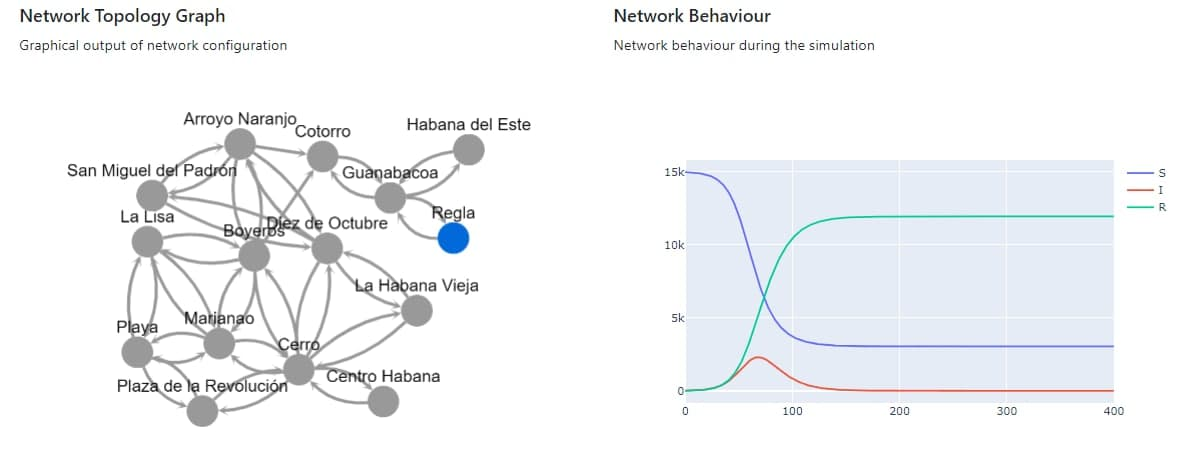
\includegraphics[width=0.7\linewidth]{test}
	\caption{Ejemplo de ejecuci\'on}

\end{figure}

Se puede seleccionar ver los resultados por cada nodo o en total. 

Los datos usados no son reales y se usaron para comprobar que el modelo resultara en un resultado sem\'antico acorde con lo esperado. Las conexiones de los nodos se escogieron de acuerdo a la siguiente figura que representa las v\'ias de comunicaci\'on entre municipios mediante las \'omnibus.

\begin{figure}[H]
	\centering
	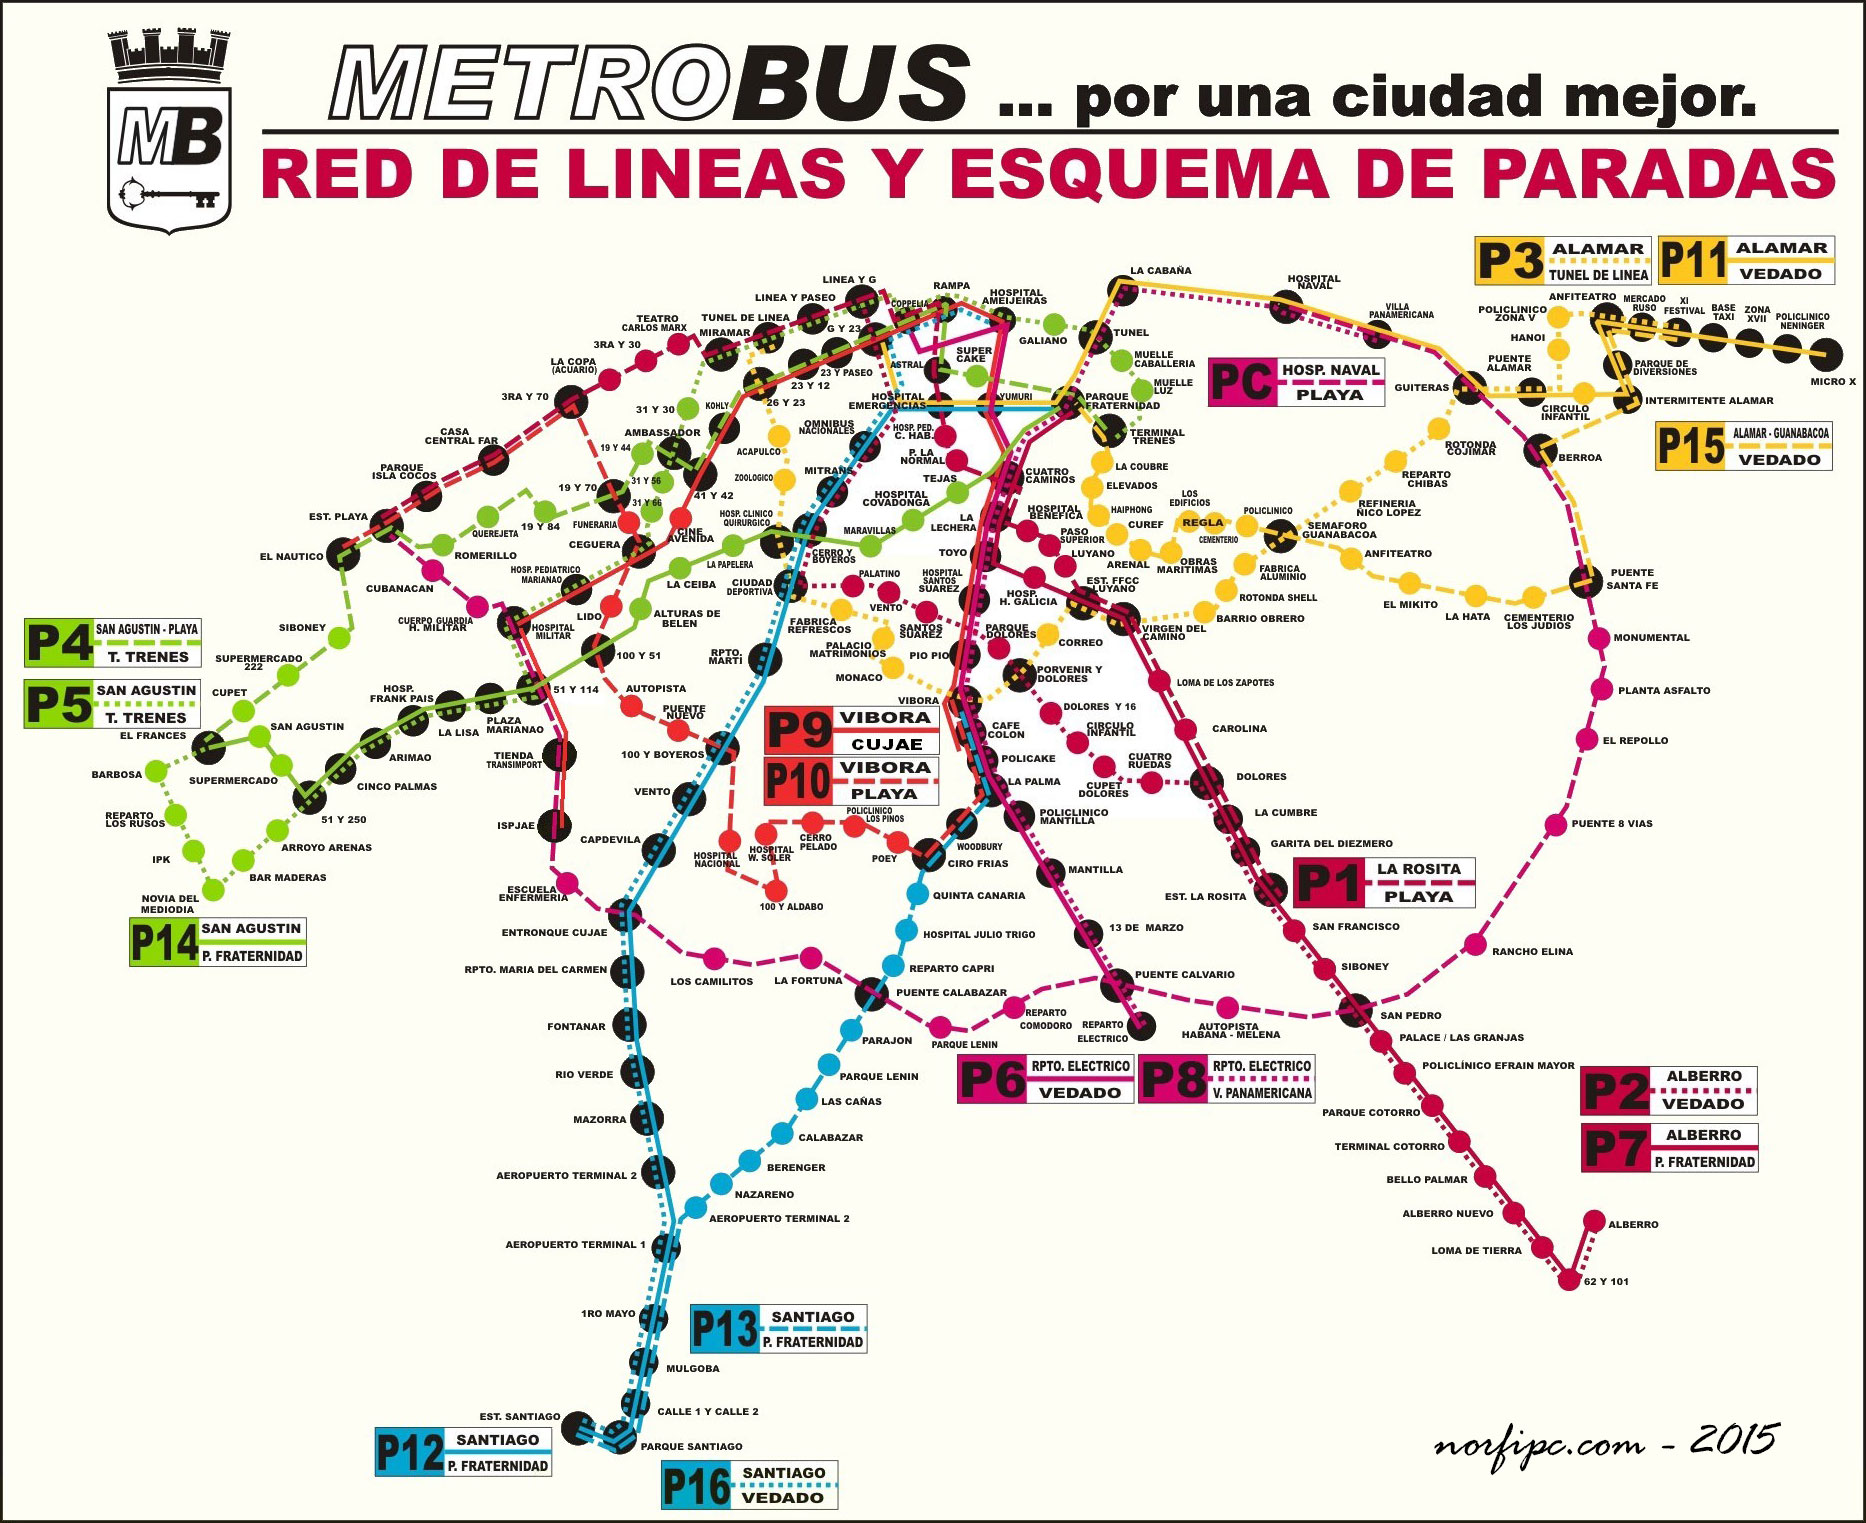
\includegraphics[width=0.7\linewidth]{map}
	\caption{Mapa de las rutas de \'omnibus de La Habana}
	\label{fig:red1---mapa-lineas-metrobus-habana}
\end{figure}

Los pesos de las aristas del grafo resultante, que significan la tasa por c\'apita en la que los individuos de un municipio visitan otro en una unidad de tiempo $t$, se asignaron acorde a la densidad que una localidad posee en cuanto a n\'umero de rutas que la atraviesan. 

Recoger datos reales para tales modelos representa un desaf\'io, pues se requiere que se midan muchos par\'ametros alrededor de toda la ciudad; como n\'umero de personas diarias que pasan por una parada, cantidad de \'omnibus disponibles por cada tipo de \'omnibus, tiempo en que se demora en viajar cada \'omnibus entre un municipio y otro, entre otras.

Por lo que para realizar pruebas para el funcionamiento de la aplicaci\'on, al menos sem\'anticamente, los datos fueron escogidos como se explica anteriormente. Se hicieron varias pruebas con diferentes par\'ametros tambi\'en. Una posible soluci\'on al problema de asignaci\'on de los par\'ametros ser\'ia disponer de las curvas reales de las variables, y ajustar los par\'ametros por el m\'etodo de m\'inimos cuadrados u otro m\'etodo de ajuste de curvas. Por lo que la aplicaci\'on sigue siendo un prototipo que se debe probar en la pr\'actica.  

En toda la literatura consultada solo se encontr\'o combinaciones puntuales de modelos compartimentales con modelo de metapoblaciones. La aplicaci\'on presente en el informe toma cualquier tipo de modelo compartimental y lo combina din\'amicamente para compilar un nuevo modelo. Por lo que se podr\'ia decir que es m\'as general. En  ninguna de las literaturas consultadas se observ\'o este tipo de enfoque. Adem\'as, se hicieron pruebas con los mismos modelos compartimentales y topolog\'ia de la red que otros art\'iculos y coinciden con los resultados que se exponen en dichos art\'iculos.

En cuanto a rendimiento, el programa es capaz de parsear modelos de distinta complejidad como SIR, SIS, SIRS y que permite utilizarlo en metamodelos de forma eficiente pudiendo generar y simular sistemas de hasta 900 ecuaciones en menos de 1 minuto. Este es el caso del sistema de \'omnibus de La Habana, que al tener 15 nodos, se puede llegar hasta  $15^2 * 4$ ecuaciones.


%===================================================================================
% Conclusiones
%-----------------------------------------------------------------------------------
\section{Conclusiones}\label{sec:conc}

Se logr\'o simular una epidemia mediante varios modelos compartimentales en combinaci\'on con modelos de metapoblaciones. La aplicaci\'on exhibe flexibilidad en cuanto a seleccionar los modelos a simular y la entrada de datos cuando una red alcanza una escala mayor. Al implementar el sistema en casos reales, se podr\'ian realizar varias simulaciones para determinar si cortando el paso entre algunas localidades se logra controlar la epidemia en cuesti\'on. La alta dimensionalidad de los modelos podr\'ia ser un problema y hubiese que recurrir a un poder de c\'omputo m\'as potente. Además, el modelo se puede generalizar para incluir otros factores, como el efecto de la inmunidad colectiva y el papel de la vacunación, a medida que los países toman las medidas necesarias para volver a la nueva normalidad.

%===================================================================================



%===================================================================================
% Recomendaciones
%-----------------------------------------------------------------------------------
\section{Limitaciones y recomendaciones}\label{sec:rec}

Entre las limitaciones podemos encontrar el uso de modelos que tengan distintos conjuntos, siendo
posible utilizar redes con distintos modelos compartimentales en los nodos estos deben cumplir
poseer los mismos conjuntos. Esta limitación pudiese abordarse desde el enfoque de que todos los
nodos tienen los mismos conjuntos sin embargo plantea grandes retos, por ejemplo si población
vacunada pasa de un nodo a otro que no tiene dicho conjunto cómo debería ser el comportamiento
del conjunto en este nuevo nodo.
Otra limitación importante es que debido a que los modelos son procesados simbólicamente
durante la compilación puede darse el caso donde conjuntos con símbolos distintos tienen un
mismo significado semántico sin embargo la aplicación no tiene forma de reconocer esto por lo que
es necesario un uso consciente de la notación por parte del usuario.
Algunas adiciones interesantes podrían ser nuevos modelos de redes o meta modelos como redes
con varios niveles o extender el modelo Simple Trip para un viaje de k nodos.

%===================================================================================



%===================================================================================
% Bibliografía
%-----------------------------------------------------------------------------------
\begin{thebibliography}{99}
%-----------------------------------------------------------------------------------	
	\bibitem{Arino} Arino and van den Driessche. \emph{A multi-city epidemic model}.
	\bibitem{Citron} Daniel T. Citron. \emph{Comparing metapopulation dynamics of infectious diseases under different models of human movement}.
	\bibitem{Martcheva} Martcheva. \emph{An Introduction to Mathematical Epidemiology}. 2015
	\bibitem{Aleta} Aleta Casas. \emph{Modelos metapoblacionales para la difusión de epidemias}. 2014
	
%-----------------------------------------------------------------------------------
\end{thebibliography}

%-----------------------------------------------------------------------------------

\label{end}

\end{document}

%===================================================================================
